\addbibresource{reference.bib}

\chapter{Master}\label{chap:master}
V této kapitole bude čtenář podrobněji seznámen s masterem -- centrálním řídícím prvkem systému Pixnet. Hlavním úkolem masteru je řízení handlerů (viz \ref{chap:handler}), persistence konfigurace a poskytování REST API pro své řízení. Primárním konzumentem API je webová frontend aplikace, poskytující uživatelské rozhraní pro řízení systémů jeho operátorem, pomocí poskytovaného API může být ale řízení systému integrováno i do systémů třetích stran\footnote{Např. DCS v CERN, jak již bylo popsáno v kapitole \ref{chap:arch:hw}}.

Tato komponenta se skládá ze dvou nezávislých částí -- backendového serveru (\ref{chap:master:backend}) frontendového webového klienta (\ref{chap:master:frontend}).

%********************************************************************************
% Backend
%********************************************************************************
\section{Backend}\label{chap:master:backend}
Backendová aplikace mastera, podobně jako handlera, byla implementována pomocí Spring Boot frameworku (viz \ref{chap:arch:technologie:spring}) a obsahuje embedovaný webový server \texttt{Tomcat}. Aplikace komunikuje s handlery, jejichž prostřednictvím řídí jim přiřazené detektory.

\subsection{Softwarová architektura}\label{chap:master:backend:sw_arch}
Na obrázku \ref{fig:master:arch} je znázorněna softwarová architektura backendové aplikace mastera, rozdělená do několika vrstev, které budou v následujících podkapitolách blíže vysvětleny.

\begin{figure}[h]
	\begin{center}
		\vspace*{0.4cm}
		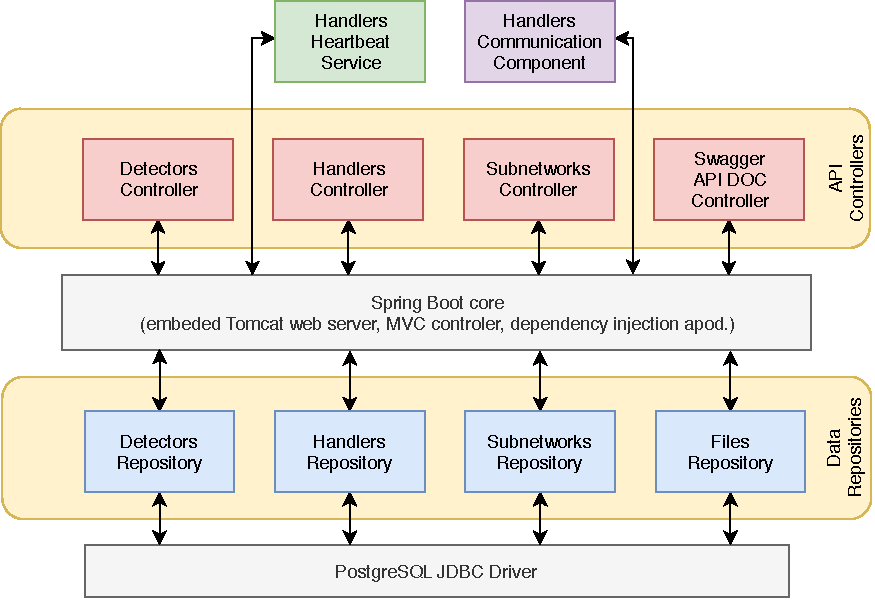
\includegraphics[width=14cm]{figures/master_arch.pdf}
		\caption{Pixnet -- master: softwarová architektura s vrstvami pro (i) persistenci konfiguraci s stavu systému (\textit{Data Repositories}), (ii) poskytování API (\textit{API controllers}),(iii) komponentu pro komunikaci s handlery (\textit{Handlers Communication Component}) a (iv) službu pro pravidelnou aktualizaci stavu handlerů (\textit{Handler Heartbeat Service}).}
		\label{fig:master:arch}
	\end{center}
\end{figure}

\subsubsection{Vrstva pro persistenci konfigurace a stavu systému}
Tato vrstva je zodpovědná za komunikaci s \textit{PostgreSQL} databází (viz \ref{chap:arch:technologie:postgresql}) pomocí \textit{PostgreSQL} \texttt{JDBC}\footnote{Z angl. \textit{Java Database Connectivity} -- API pro programovací jazyk Java, definující přístup klienta k databázi.} ovladače. Pro mapování jednotlivých entit (resp. Java objektů, tzv. \texttt{ORM}\footnote{Z angl. \textit{Object-relational mapping} -- objektově-relační mapování.}) byl implementován framework \textit{Hibernate}.

Vrstva poskytuje repozitáře (viz obr. \ref{fig:master:arch}) pro dotazy nad uloženými daty a pro jejich modifikaci. Rovněž je zodpovědná za automatické vytváření a aktualizaci databázového schématu, připojené databáze. Návrh schématu bude popsán v \ref{chap:master:backend:db}.

V databázi jsou společně se záznamem detektoru uloženy také jeho moduly (resp. implementace komunikačního a datového interface).

\subsubsection{Komponenta pro komunikaci s handlery}
Komponenta poskytuje metody pro komunikaci s handlery pomocí jejich API, popsaném v \ref{tab:handler:api_detectors}. Umožňuje přiřazování detektorů jednotlivým handlerům, navazování spojení s detektory, zjišťování jejich stavu a funkcionality (vč. seznamů podporovaných příkazů), vykonávání jednotlivých příkazů, nahrávání souborů apod.

\subsubsection{Vrstva s API kontroléry}\label{chap:master:backend:sw_arch:api}
Tato vrstva se sestává z REST API kontrolérů pro poskytování API metod pro řízení mastera. Těmito kontroléry jsou:
\begin{description}
    \item[\texttt{Subnetworks Controller}] -- poskytuje CRUD\footnote{Z angl. \textit{Create Read Update and Delete}, operace pro vytváření, čtení, aktualizaci a odstranění.} operace nad entitou podsítí (viz \ref{chap:arch:hw}). Pro přehled endpointů viz tabulka \ref{tab:master:api_subnetworks}.

    \begin{table}[h!]
        \begin{center}
            \begin{tabular}{|c|c|l|}
                \hline
          \textbf{HTTP} & & \\
          \textbf{Metoda} & \textbf{Endpoint} & \textbf{Popis} \\
            \hline
            POST & \texttt{/add} & Přidá novou podsíť \\
            GET & \texttt{/getAll} & Vrátí seznam všech podsítí \\
            DELETE & \texttt{/deleteAll} & Odstraní všechny podsítě \\
            DELETE & \texttt{/deleteById} & Odstraní podsíť podle zadaného ID \\
            \hline
            \end{tabular}
        \end{center}
        \caption{Endpointy komponenty \textit{Subnetworks Controller} (všechny endpointy mají prefix \texttt{/api/subnetwork}).}
        \label{tab:master:api_subnetworks}
    \end{table}

    \item[\texttt{Handlers Controller}] -- poskytuje CRUD operace nad entitou handlerů. Pro přehled endpointů viz tabulka \ref{tab:master:api_handlers}.

    \begin{table}[h!]
        \begin{center}
            \begin{tabular}{|c|c|l|}
                \hline
          \textbf{HTTP} & & \\
          \textbf{Metoda} & \textbf{Endpoint} & \textbf{Popis} \\
            \hline
            POST & \texttt{/add} & Přidá nový handler \\
            GET & \texttt{/getAll} & Vrátí seznam všech handlerů \\
            DELETE & \texttt{/deleteAll} & Odstraní všechny handlery \\
            DELETE & (pouze prefix) & Odstraní handler podle zadaného ID \\
            \hline
            \end{tabular}
        \end{center}
        \caption{Endpointy komponenty \textit{Handlers Controller} (všechny endpointy mají prefix \texttt{/api/handler}).}
        \label{tab:master:api_handlers}
    \end{table}

    \item[\texttt{Detectors Controller}] -- kromě poskytování CRUD operací nad entitou detektorů také poskytuje metody pro přiřazování detektorů handlerům, navazování spojení s detektory, vykonávání jejich příkazů (viz \textit{ValueCommands} a \textit{ExecutionCommands}, \ref{chap:handler:detector_layer:commIntf}). Pro přehled endpointů viz tabulka \ref{tab:master:api_detectors}.

    \begin{table}[h!]
        \begin{center}
            \begin{tabular}{|c|c|l|}
                \hline
          \textbf{HTTP} & & \\
          \textbf{Metoda} & \textbf{Endpoint} & \textbf{Popis} \\
            \hline
            POST & \texttt{/add} & Přidá nový detektor \\
            GET & \texttt{/getAll} & Vrátí seznam všech detektorů \\
            GET & \texttt{/getById} & Vrátí jeden detektor \\
            GET & \texttt{/getDetailById} & Vrátí detail jednoho detektoru \\
            DELETE & (pouze prefix) & Odstraní detektor podle zadaného ID \\
            POST & \texttt{/bindToHandler} & Přiřadí detektor handleru \\
            POST & \texttt{/unbindFromHandler} & Odebere detektor handleru \\
            POST & \texttt{/connect} & Naváže spojení mezi handlerem a detektorem \\
            POST & \texttt{/disconnect} & Ukončí spojení mezi handlerem a detektorem \\
            POST & \texttt{/executeValueCommand} & Vykoná \texttt{ValueCommand} detektoru \\
            POST & \texttt{/executeExecutionCommand} & Vykoná \texttt{ExecutionCommand} detektoru \\
            POST & \texttt{/uploadFile} & Nahraje soubor do detektoru \\
            \hline
            \end{tabular}
        \end{center}
        \caption{Endpointy komponenty \textit{Detectors Controller} (všechny endpointy mají prefix \texttt{/api/detector}).}
        \label{tab:master:api_detectors}
    \end{table}    

    \item[\texttt{Swagger API DOC Controller}] -- kontrolér pro poskytování webové API dokumentace, dostupné z endpointu \texttt{/apiDoc}. Tato komponenta byla implementována, podobně jako u handleru (viz \ref{chap:handler:spring:swagger}), za pomocí \textit{Springfox} \cite{springfox} knihovny. Kromě přehledu všech endpointů webové rozhraní také poskytuje definici datového modelu API (ve formátu JSON) a umožňuje manuální volání jednotlivých endpointů. Endpoint pro stažení Open\-API specifikace ve formátu JSON je \texttt{/v2/api-docs}.
\end{description}

\subsubsection{Handlers Heartbeat Service}
Tato služba slouží k periodickému zjišťování stavu jednotlivých handlerů (a tranzitivně i detektorů) systému. V pravidelných intervalech (defaultně nastaveno na \unit{10}{s}) je navázáno spojení se všemi handlery pomocí jejich \texttt{/status} endpointu (viz \ref{chap:handler:spring:status_api}) a jsou aktualizována stavová data v databázi.

\subsection{Návrh databáze}\label{chap:master:backend:db}
Na obrázku \ref{fig:master:db_schema} je znázorněno schéma relačního modelu \textit{PostgreSQL} databáze, kde jsou znázorněny jednotlivé entity, vč. jejich atributů, a relace mezi nimi pomocí cizích klíčů.

Ve schématu jsou dále definována různá integritní omezení, která vynucují strukturu dat a pravidla mezi relacemi entit -- např. že handler musí mít přiřazení právě jednu podsíť, že detektor může být přiřazen handleru ze stejné podsítě apod.

\begin{figure}[h]
	\begin{center}
		\vspace*{0.4cm}
		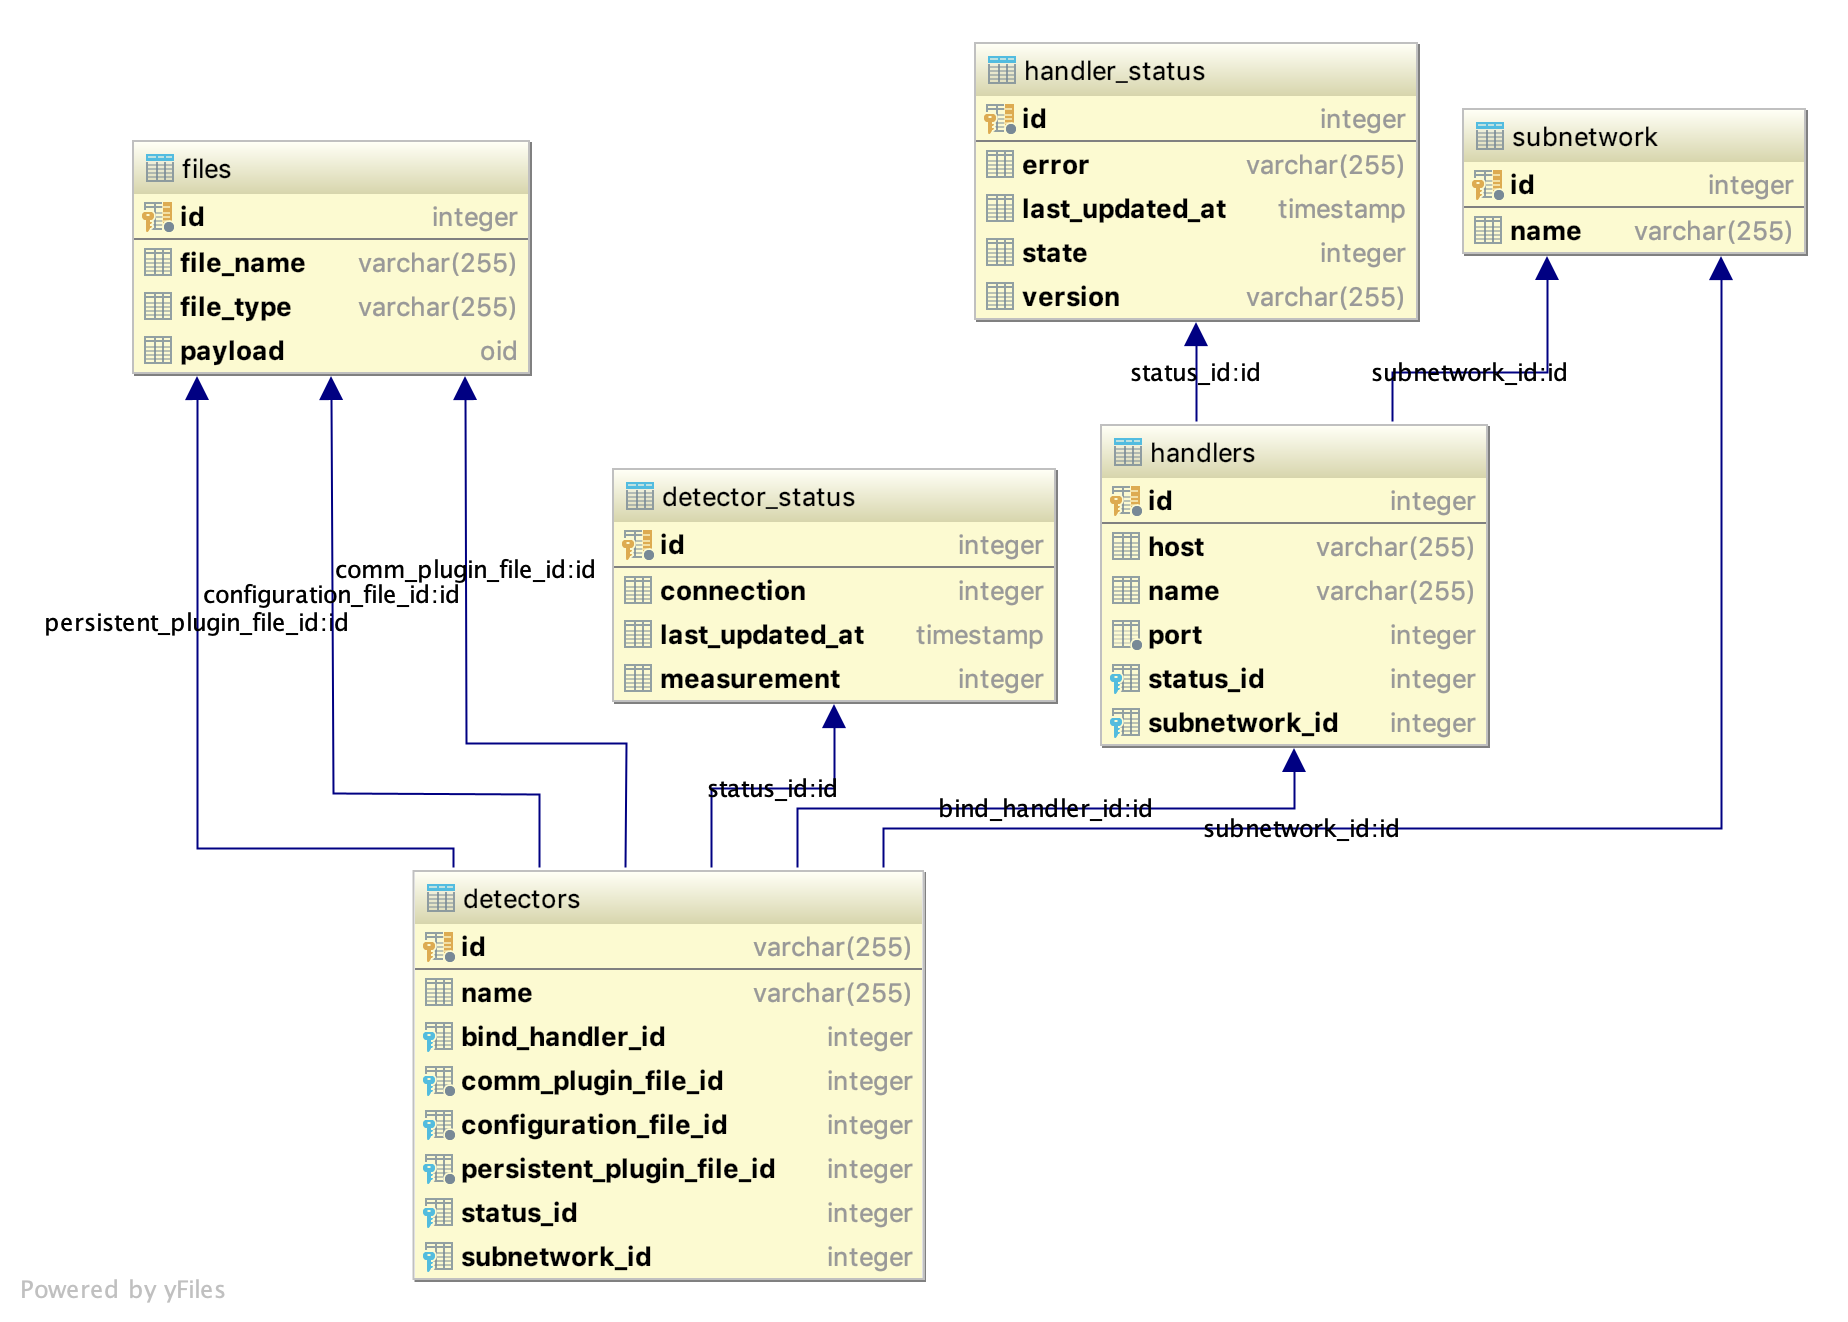
\includegraphics[width=15cm]{figures/master_db.png}
		\caption{Pixnet -- master: databázové schéma.}
		\label{fig:master:db_schema}
	\end{center}
\end{figure}

\subsection{Konfigurace a nasazení}
Pro spuštění mastera je třeba mít nainstalované \texttt{JRE 8}\footnote{\textit{Java SE Runtime Environment, dostupné z\\\url{https://www.oracle.com/technetwork/java/javase/downloads}}.} nebo vyšší.
Zkompilovanou java aplikaci je třeba spustit s argumentem \texttt{masterConfig} obsahující cestu ke konfiguračnímu souboru (pro příklad viz zdrojový kód \ref{src:master:config}), obsahujícího port na kterém bude aplikace naslouchat příchozí spojení.

Aplikaci je tedy možné spustit například takto: \mint{bash}{java -jar master.jar masterConfig=config.yaml}

\begin{code}[h]
  \begin{minted}[
  frame=single,
  linenos,
  breaklines
  ]{yaml}
# Connection parameters
portToListen: 8080
\end{minted}
\caption{\texttt{YAML} konfigurační soubor mastera.}
\label{src:master:config}
\end{code}

%********************************************************************************
% Frontend
%********************************************************************************
\section{Frontend}\label{chap:master:frontend}
Pomocí frameworku \textit{ReactJS} (viz \ref{chap:arch:technologie:react}) byl implementován webový klient, který implementuje API, poskytované backendovou aplikací mastera (viz \ref{chap:master:backend:sw_arch:api}). 

Jedná se o tzt. \textit{single-page} aplikaci, tj. aplikaci která načte jednu stránku, kterou pak dynamicky aktualizuje dle interakcí uživatele (ev. dalších událostí) bez nutnost stahování nové stránky ze serveru. Jak již bylo vysvětleno v kapitole \ref{chap:arch:technologie:react}, každá \textit{ReactJS} aplikace je založena na komponentách. Každá komponenta má svoje vlastnosti a svůj stav. Komponenty lze opětovně používat a je možné je libovolně zapouzdřovat. Při aktualizaci stavu některé z komponent, \textit{ReactJS} framework změnu detekuje a provede překreslení afektovaných částí uživatelského rozhraní.

Pro navigaci po stránce aplikace používá knihovnu \textit{react-router}\footnoteUrl{https://reacttraining.com/react-router/web}, která mění obsah stránky renderováním těchto komponent:

\begin{description}
    \item[Subnetworks] -- komponenta vizualizující seznam podsítí a umožňuje přidávání nových podsítí a odebírání existujících.
    \item[Handlers] -- tato komponenta zobrazuje seznam přidaných handlerů, včetně podseznamu jim přiřazených detektorů, stavu apod. Komponenta rovněž umožňuje přidání nových hadlerů a odstranění existujících. Pro screenshot viz obr. \ref{fig:master:frontend:handlers}.
    \item[Detectors] -- komponenta zobrazující seznam všech detektorů (viz \ref{fig:master:frontend:detectors}). Dále umožňuje přidávání nových detektorů a odebírání existujících.
    \item[Detector detail] -- komponenta s detailem detektoru (viz obr. \ref{fig:master:frontend:detector_detail}). Komponenta uživateli nabízí všechny operace nad detektorem, nabízené API backendové aplikace mastera (tj. např. přiřazování detektoru dostupnému handleru, navazování spojení s detektorem, vykonávání jeho příkazů apod.).
\end{description}

\begin{figure}[h]
	\begin{center}
        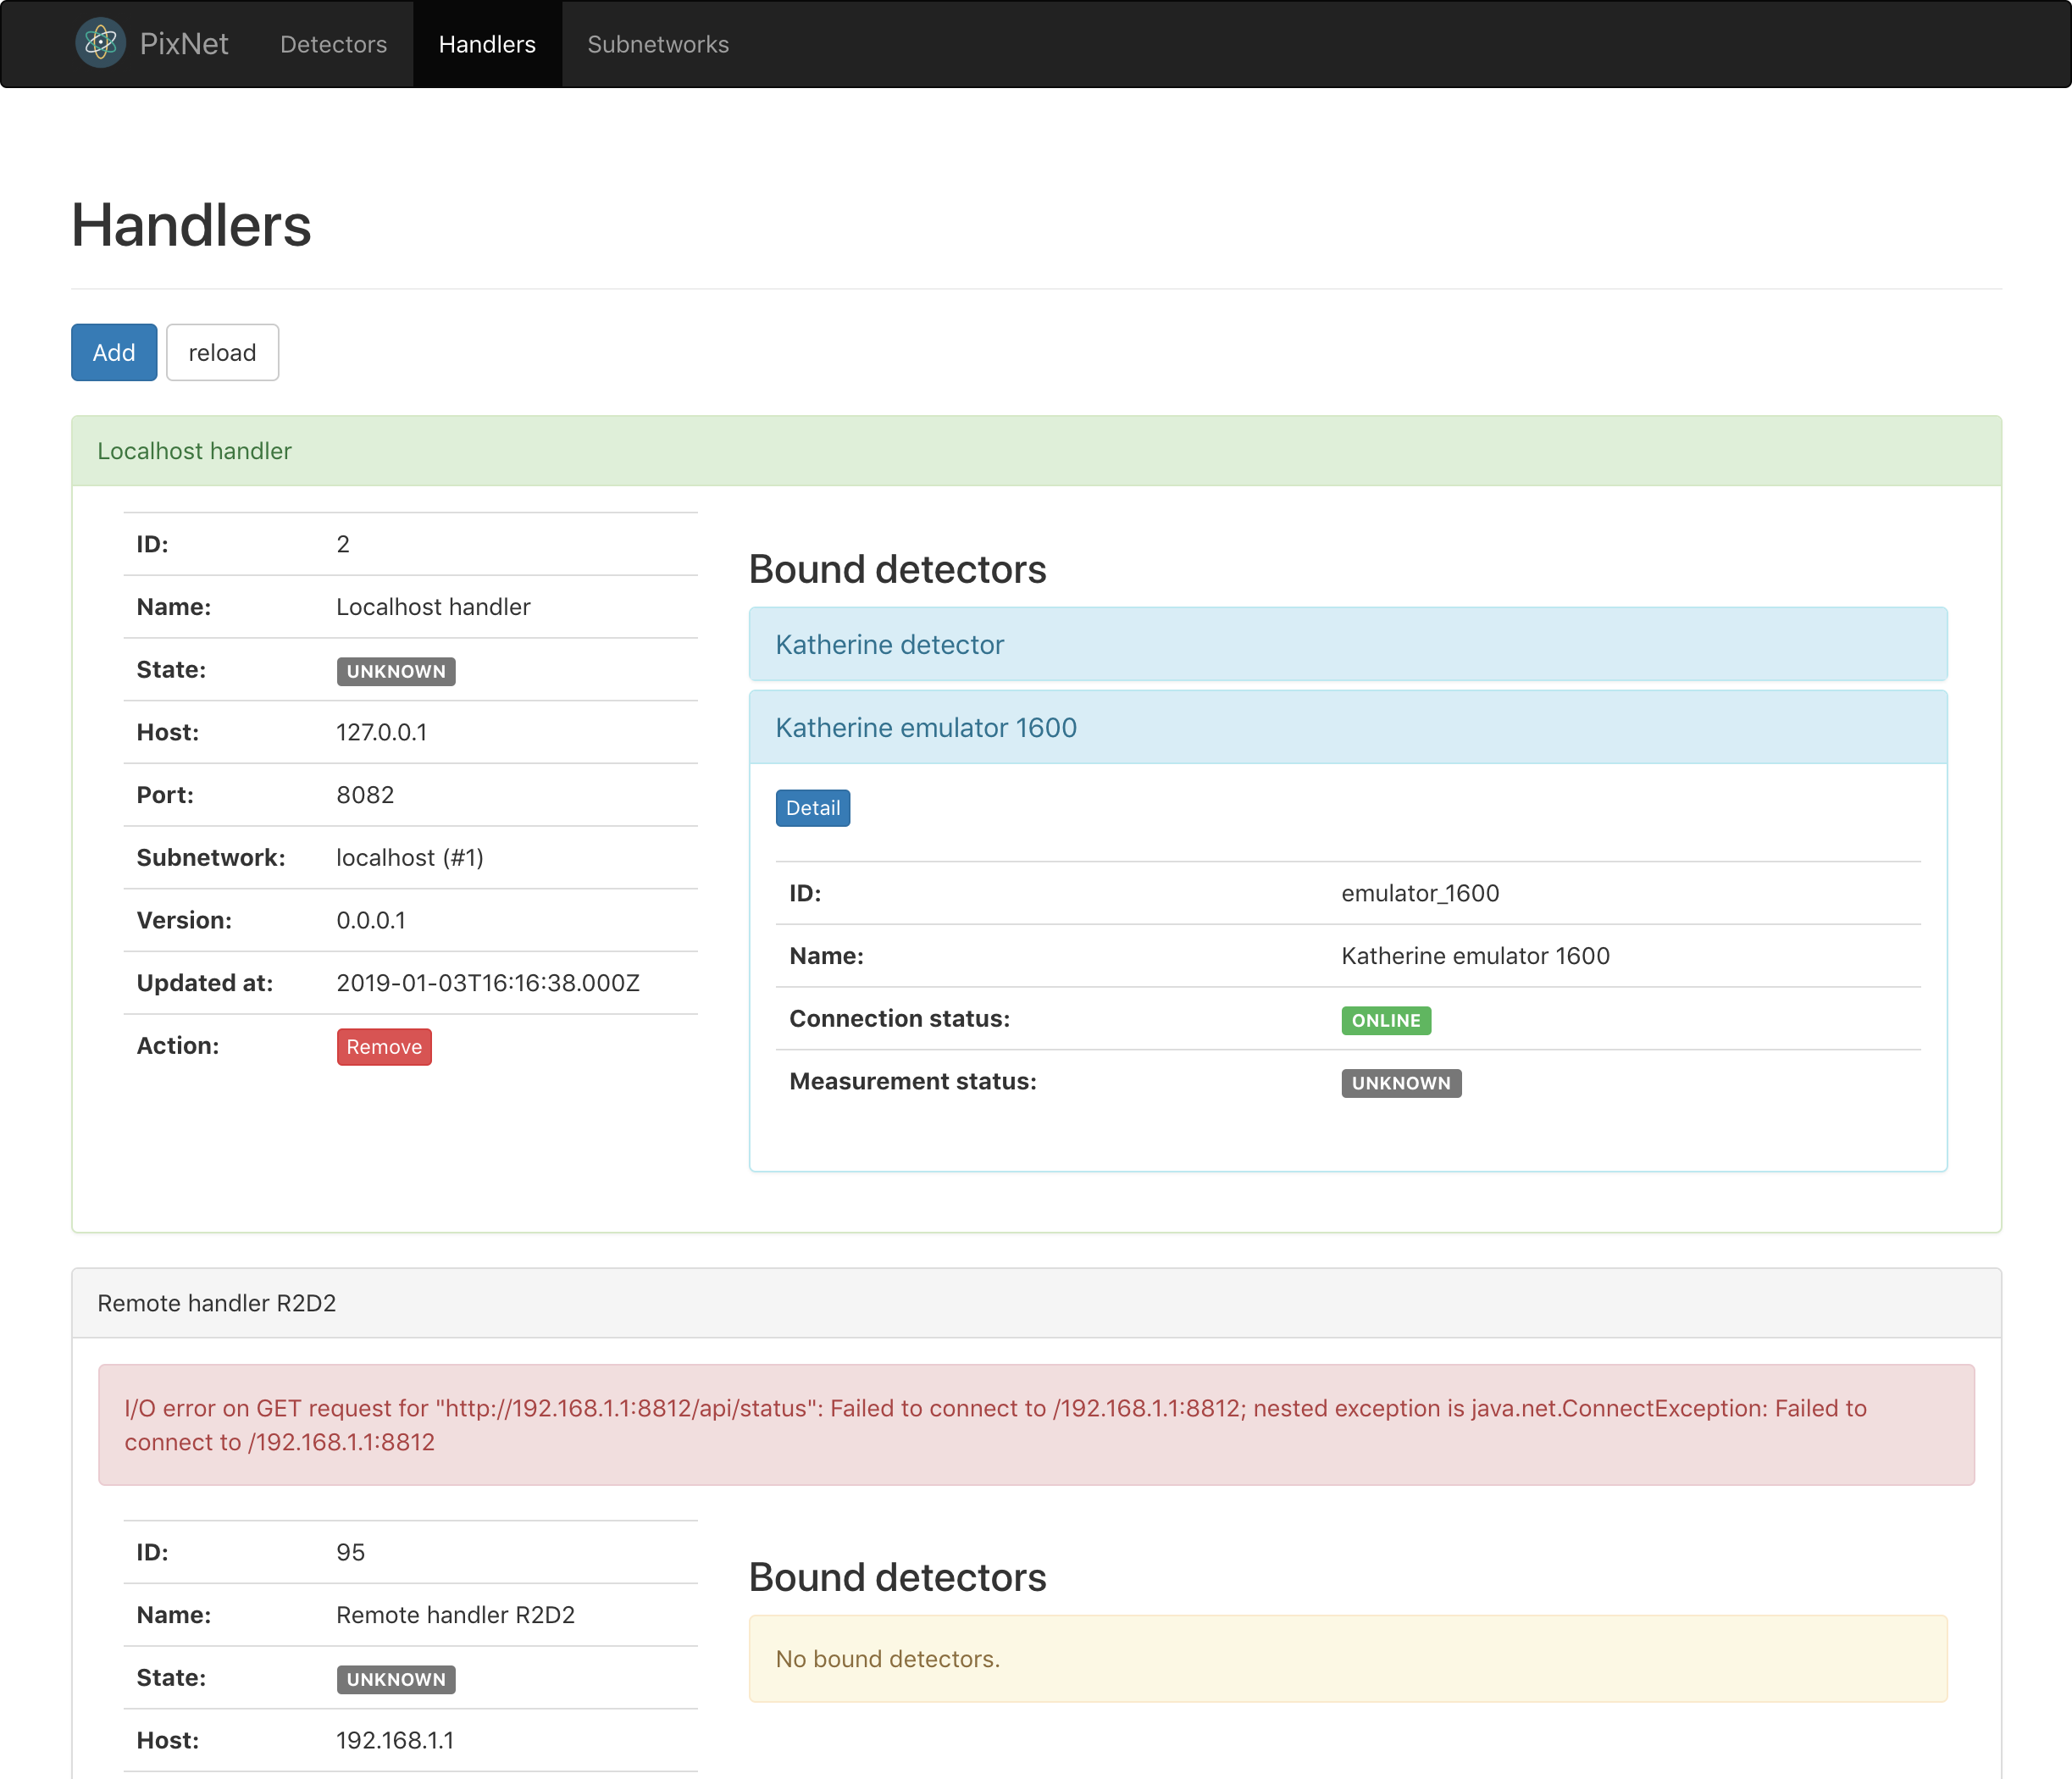
\includegraphics[width=15cm]{figures/master_handlers.png}
	\end{center}
	\caption{Master -- frontend: screenshot seznamu handlerů, dostupného z endpointu \texttt{/handlers}.}
	\label{fig:master:frontend:handlers}
\end{figure}

\begin{figure}[h]
	\begin{center}
        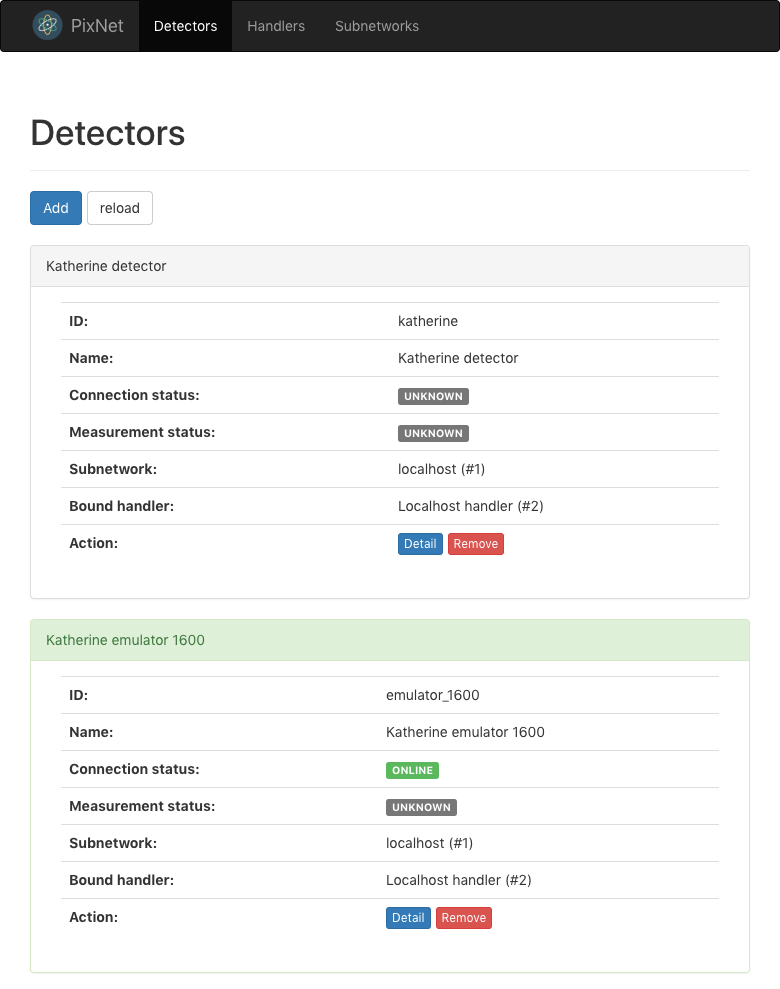
\includegraphics[width=10cm]{figures/master_detectors.png}
	\end{center}
	\caption{Master -- frontend: screenshot seznamu detektorů, dostupného z endpointu \texttt{/detectors}.}
	\label{fig:master:frontend:detectors}
\end{figure}

\begin{figure}[h]
	\begin{center}
        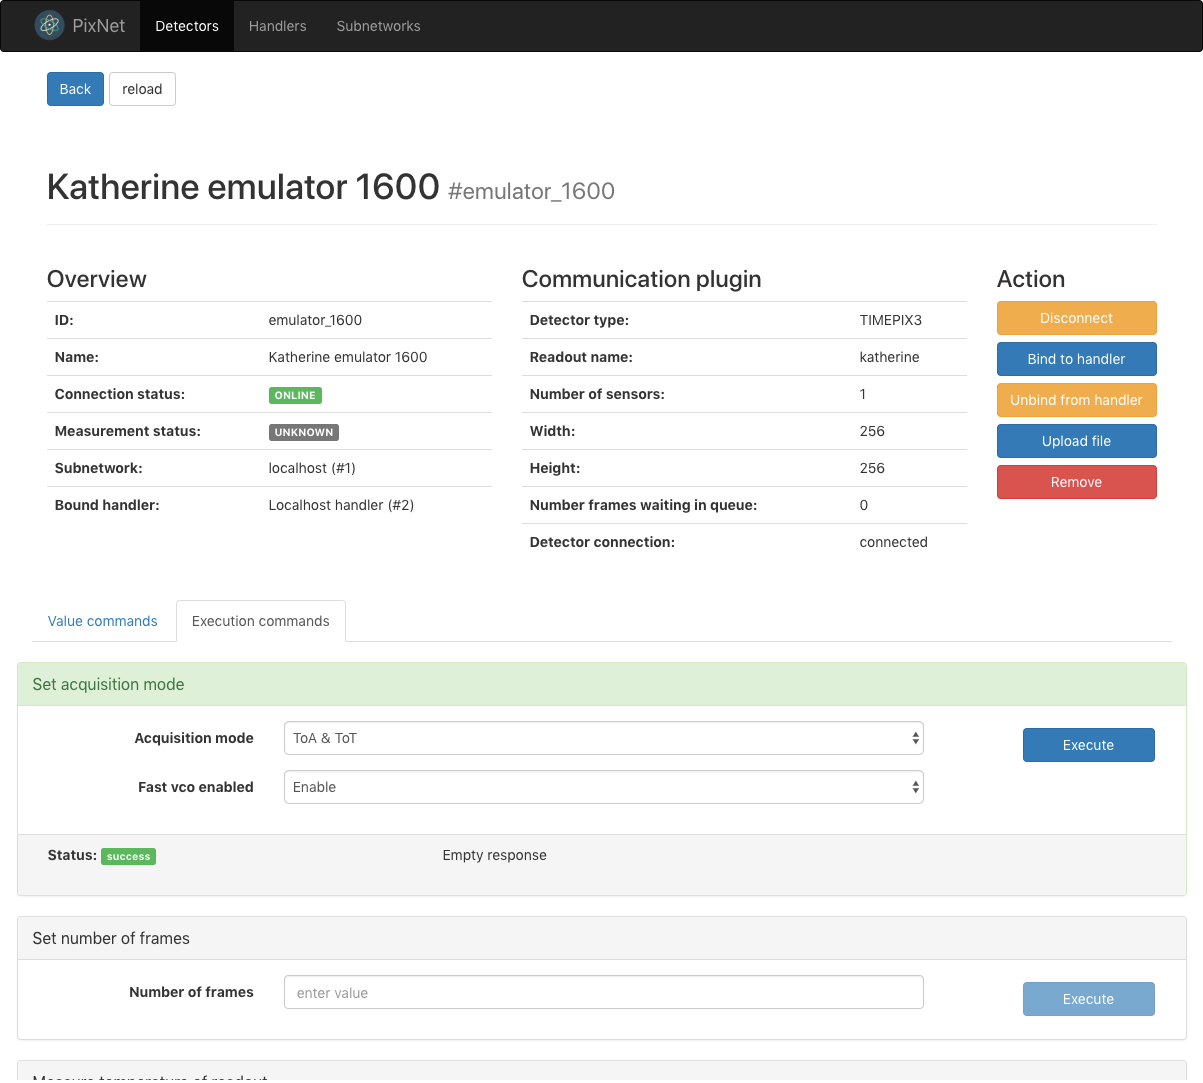
\includegraphics[width=15cm]{figures/master_detector_detail.png}
	\end{center}
    \caption{Master -- frontend: screenshot detailu detektoru, dostupného z endpointu \texttt{detectors/\{ID detektoru\}}.}
	\label{fig:master:frontend:detector_detail}
\end{figure}

\subsection{Nasazení}
Nasazení aplikace je jednoduché -- stačí jenom její build (k dispozici na přiloženém CD) nahrát na webový server. Build obsahuje \texttt{index.html} společně s vlastní aplikací v \texttt{bundle.js} a dalšími soubory (obrázky, CSS styly apod.).

Aplikace byla vyvinuta pomocí systému na správu závislostí \texttt{Yarn}\footnoteUrl{https://yarnpkg.com}. Pro vývojové účely je možné aplikaci spustit příkazem \texttt{yarn start}, nebo příkazem \texttt{yarn build} je možné udělat build aplikace, nasaditelný na webový server.